\section{BAYESIAN DEEP LEARNING}

\begin{yellowbox}{\textbf{NOMENCLATURE}}
    \begin{tabularx}{\columnwidth}{ll}
        $$ & \\
        \addlinespace[2pt]
        $$ & \\
        $$ & \\
        $$ & \\
        $$ & \\
        $$ & \\
        $$ & \\
        $$ & \\
        $$ & \\
   
    \end{tabularx}
\end{yellowbox}

\begin{whitebox}{\textbf{BAYESIAN NEURAL NETWORKS}}
    \begin{itemize}
        \item Modern NNs show strong performance in complex decision making but generally tend to be overconfident in their predictions ($\to$ calibration)
        \item Prior over weights $\bm{\theta}$ e.g. Gaussian $p(\bm{\theta})=\mathcal{N}(\bm{\theta};\bm{0},\sigma^2\mathbb{I})$
        \item Likelihood function parameterized by neural network $\bm{f}$
        \begin{align*}
            p(y_{1:n}\mid\bm{x}_{1:n},\bm{\theta})=\prod_{i=1}^np(y_i\mid\bm{x}_i,\bm{\theta})=\prod_{i=1}^np(y_i\mid\bm{f}(\bm{x}_i;\bm{\theta}))
        \end{align*}
        \item Posterior
        \begin{align*}
            p(\bm{\theta}\mid\bm{x}_{1:n},y_{1:n})=\frac{1}{Z}p(\bm{\theta})p(y_{1:n}\mid\bm{x}_{1:n},\bm{\theta})
        \end{align*}
        where
        \begin{align*}
            Z=p(y_{1:n}\mid\bm{x}_{1:n})=\int p(\bm{\theta})p(y_{1:n}\mid\bm{x}_{1:n},\bm{\theta})\ d\bm{\theta}
        \end{align*}
        is the \textit{intractable} marginal likelihood for NNs (as modern NNs have millions to billions of parameters)
        \item Maximum a posteriori (MAP) is a typical neural network objective
        \begin{align*}
            \hat{\bm{\theta}}=\arg\max_{\bm{\theta}}\log p(\bm{\theta})+\sum_{i=1}^n\log p(y_i\mid\bm{x}_i,\bm{\theta})
        \end{align*}
        \begin{itemize}
            \item Optimization using SGD variants (no closed form solution)
            \item MAP is only a point estimate (Dirac posterior approximation)
            \begin{align*}
                p(\bm{\theta}\mid y_{1:n},\bm{x}_{1:n})\approx\delta(\bm{\theta}=\hat{\bm{\theta}})
            \end{align*}
            \item Posterior $p(\bm{\theta}|\mathcal{D})$ (where $\mathcal{D}$ denotes the data set $y_{1:n},\bm{x}_{1:n}$) is just the normalized joint distribution $p(\bm{\theta},\mathcal{D})$
            \item Posterior captures the entire loss landscape, MAP only a single point
            \resizebox{0.9\linewidth}{!}{
                \includegraphics[
                page=8,
                trim = {0.5cm, 1.5cm, 0.5cm, 2.5cm}, % left, bottom, right, top
                clip
                ]{media/23HS_Tut07_BDL.pdf}
            }
        \end{itemize}
        \item Inference
        \begin{itemize}
            \item Predictive Posterior for a new input $\bm{x}^*$ by marginalizing out the posterior
            \begin{align*}
                p(y^*\mid\bm{x}^*,\mathcal{D})=\int p(y^*\mid\bm{x}^*,\bm{\theta})\ p(\bm{\theta}\mid\mathcal{D})\ d\bm{\theta}
            \end{align*}
            \begin{itemize}
                \item This forms a Bayesian model average of infinitely many models weighted by their posterior probabilities
                \item The MAP is a single point estimate
            \end{itemize}
            \item Training and evaluating an ordinary NN with dropout can be interpreted as performing approximate inference on a BNN
        \end{itemize}
    \end{itemize}
\end{whitebox}

\begin{whitebox}{\textbf{APPROXIMATE INFERENCE FOR BNNS}}
    \begin{itemize}
        \item Allows estimating the posterior and predictive distribution
        \begin{itemize}
            \item Variational inference\\
            (most commonly Gaussians $q(\bm{\theta};\lambda)=\mathcal{N}(\bm{\theta};\bm{\mu},\bm{\Sigma})$)
            \begin{itemize}
                \item Bayes by backprop
                \item Variational Gauss-Newton
                \item Monte Carlo Dropout
            \end{itemize}
            \item Laplace approximation
            \item SWA-Gaussian (SWAG)
            \item Deep ensembles
            \item MCMC
            \begin{itemize}
                \item Stochastic Gradient Langevin Dynamics
                \item Hamiltonian Monte Carlo
            \end{itemize}
        \end{itemize}
    \end{itemize}
\end{whitebox}

\begin{whitebox}{\textbf{BAYES BY BACKPROP}}
    \begin{itemize}
        \item Variational family is diagonal Gaussians $\mathcal{N}(\bm{\mu},\mathbb{I}\bm{\sigma})$
        \item Maximizes the ELBO using backprop (autodiff)
        \item Algorithm
        \begin{center}
            \begin{algorithmic}
                \footnotesize
                \State $\lambda=\lambda_0=\{\bm{\mu}_0,\bm{\sigma_0}\}$
                \Comment{Input}
                % \Loop
                \For{$t=1,2,\dots$}
                %\Comment{TODO}
                \State Draw $\epsilon\sim\mathcal{N}(\bm{0},\mathbb{I})$
                \State $\bm{\theta}=t(\epsilon,\lambda)=\bm{\mu}+\bm{\sigma}\circ\epsilon$
                \State $\mathcal{L}(\lambda)=\log q(\bm{\theta};\lambda)-\log p(\bm{\theta})-\log p(\mathcal{D}\mid\bm{\theta})$
                \State $\nabla_\lambda\mathcal{L}=\mathrm{backprop}_\lambda(\mathcal{L})$
                \State $\lambda=\lambda-\alpha\nabla_\lambda\mathcal{L}$
                \EndFor
                % \EndLoop
            \end{algorithmic}
        \end{center}
        \item Can minibatch and reduce variance by using multiple $\epsilon$ samples
        \item Can perform worse than standard NNs due to change in training
    \end{itemize}
\end{whitebox}

\begin{whitebox}{\textbf{MONTE CARLO DROPOUT}}
    \begin{center}
        \resizebox{0.9\linewidth}{!}{
            \includegraphics[
            page=24,
            trim = {1.0cm, 2.0cm, 1.0cm, 2.0cm}, % left, bottom, right, top
            clip
            ]{media/23HS_Tut07_BDL.pdf}
        }
    \end{center}
    \begin{itemize}
        \item Idea: perform dropout not only during training but also during inference
        \item Can be seen as performing variational inference with a particular family
        \begin{align*}
            q(\bm{\theta}\mid\lambda)=\prod_jq_j(\theta_j\mid\lambda_j)
        \end{align*}
        where
        \begin{align*}
            q_j(\theta_j|\lambda_j)=p\delta_0(\theta_j)+(1-p)\delta_{\lambda_j}(\theta_j)
        \end{align*}
        with $p$ being the probability that weight $\theta_j$ is set to $0$ and $\lambda_j$ being the value of the weight
        \item Predictive uncertainty is approximated by averaging across samples
        \begin{align*}
            p(y^*\mid\bm{x}^*,\bm{x}_{1:n},y_{1:n})\approx\frac{1}{m}\sum_{j=1}^mp(y^*\mid\bm{x}^*,\bm{\theta}^{(j)})
        \end{align*}
        where $\bm{\theta}^{(j)}$ is the NN with certain weights set to $0$
    \end{itemize}
\end{whitebox}

\begin{whitebox}{\textbf{DEEP ENSEMBLES}}
    \begin{enumerate}
        \item Obtain MAP estimate for several neural networks, each separately trained on a different dataset obtained via bootstrap sampling (uniform sampling with replacement)
        \item Average outputs of different models to approximate predictive posterior
        \begin{itemize}
            \item Combine with variational inference, Laplace and SWAG to get mixture of Gaussian posterior approximations
        \end{itemize}
    \end{enumerate}
\end{whitebox}

\begin{whitebox}{\textbf{STOCHASTIC GRADIENT LANGEVIN DYNAMICS (SGLD)}}
    \begin{itemize}
        \item SGLD produces samples from a Bayesian posterior
        \begin{align*}
            \bm{\theta}\sim\frac{1}{Z}\exp\left(\log p(\bm{\theta})+\sum_{i=1}^n\log p(y_i\mid x_i,\bm{\theta})\right)
        \end{align*}
        as follows
        \begin{center}
            \begin{algorithmic}
                \footnotesize
                \State $\bm{\theta}=\bm{\theta}_0$
                \Comment{Input}
                % \Loop
                \For{$t=1,2,\dots$}
                %\Comment{TODO}
                \State $i_i,\dots,i_m\sim\mathrm{Uniform}(\{1,\dots,n\})$
                \State $\epsilon_t\sim\mathcal{N}(0,2\eta_t\mathbb{I})$
                \State $\bm{\theta}_{t+1}=\bm{\theta}_t-\eta_t\left(\nabla\log p(\bm{\theta}_t)+\frac{n}{m}\sum_{j=1}^m\nabla\log p(y_{i,j}\mid\bm{\theta}_t,\bm{x}_{i,j})\right)+\epsilon_t$
                \EndFor
                % \EndLoop
            \end{algorithmic}
        \end{center}
        \item Due to large number of weights, drop samples during "burn-in" period and summarize later samples via subsampling
    \end{itemize}
\end{whitebox}

\begin{whitebox}{\textbf{COMPARING APPROXIMATE INFERENCE METHODS}}
    \begin{center}
        \resizebox{0.95\linewidth}{!}{
            \includegraphics[
            page=29,
            trim = {0.5cm, 1.5cm, 0.5cm, 2.5cm}, % left, bottom, right, top
            clip
            ]{media/23HS_Tut07_BDL.pdf}
        }
    \end{center}
\end{whitebox}

\begin{whitebox}{\textbf{REGRESSION}}
    \begin{itemize}
        \item Sampling BNN weights from a learned posterior distribution $\bm{\theta}\sim q(\bm{\theta}|\lambda)$ and explicitly modeling the heteroscedastic noise in our observations allows estimating epistemic and aleatoric uncertainty
        \item Predicted mean $\mu(\bm{x},\bm{\theta})$ and variance $\sigma(\bm{x},\bm{\theta})^2$ describe the output distribution
        \item Mean predicted output
        \begin{align*}
            \mathbb{E}[y^*|\bm{x}^*]\approx\bar{\mu}(\bm{x}^*):=\frac{1}{m}\sum_{j=1}^m\mu\left(\bm{x}^*,\bm{\theta}^{(j)}\right)
        \end{align*}
        \begin{center}
            \resizebox{0.90\textwidth}{!}{$
            \begin{aligned}
                \mathrm{Var}[y^*|\bm{x}^*]&=\mathbb{E}[\mathrm{Var}[y^*|\bm{x}^*,\bm{\theta}]]+\mathrm{Var}[\mathbb{E}[y^*|\bm{x}^*,\bm{\theta}]]\\
                &\approx\underbrace{\frac{1}{m}\sum_{j=1}^m\sigma^2\left(\bm{x}^*,\bm{\theta}^{(j)}\right)}_{\text{Aleatoric uncertainty}}+\underbrace{\frac{1}{m}\sum_{j=1}^m\left(\mu\left(\bm{x}^*,\bm{\theta}^{(j)}\right)-\bar{\mu}(\bm{x}^*)\right)^2}_{\text{Epistemic uncertainty}}
            \end{aligned}$}    
        \end{center}
    \end{itemize}
\end{whitebox}